\documentclass[10pt]{proc}
\usepackage[fleqn]{amsmath}
\usepackage{amsfonts}
\usepackage[utf8]{inputenc}
\usepackage{amssymb}
\usepackage{listings}
\usepackage{graphicx}
\usepackage[utf8]{inputenc} 
\usepackage[top=2cm, left=2.5cm]{geometry}
\title{Oma Christels Eier-Nuss-Schokolade-Sahne-Likör-Kuchen}
\author{}
\begin{document}
\maketitle

\textbf{Dauer: etwa 1h}
\section{Zutaten}
\begin{itemize}
	\item 5 Eier
	\item 250gr Zucker, die Hälfte davon Puderzucker
	\item 200gr geriebene Haselnüsse
	\item 100gr gemahlene Mandeln
	\item 150gr Zartbitterschokolade
	\item 2 Tropfen Bittermandelöl
	\item 1 Messerspitze Backpulver
	\item 1 Glas Sauerkirschen
	\item 1 Packung Vanillepudding
	\item 500ml Sahne
	\item 1 Fläschchen Eierlikör
\end{itemize}

\section{Boden}
\begin{itemize}
	\item Eier mit Zucker schaumig schlagen, das dauert ca 5-10 min
	\item Schokolade zu kleinen Stücken reiben/hacken
	\item In die schaumige Eimasse die Nüsse, Schokolade, 1 Messerspitze Backpulver geben
	\item 2 bis 3 Tropfen Bittermandelöl hinzugeben und gut einrühren. NICHT MEHR !
\end{itemize}
Den Teig in eine gut eingefettete Form gießen und bei 180C abbacken. Zwischendurch kontrollieren, der Teig sollte nicht braun werden, muss aber trocknen. Dazu während dem Backvorgang Löcher einstechen. Dauer ca: 20 min.
\\
\textbf{Teig abkühlen lassen}.
\section{Kirschen}
Die Kirschen mit Flüssigkeit in einen Topf geben und langsam erwärmen. Puddingpulver und ein bischen Zucker einrühren, halbe Minute aufkochen lassen.\\
Noch warm auf dem Kuchen verteilen.

\section{Kurz vor dem Verzehr}
Sahne schlagen und auf dem Kuchen verteilen. Auf der Sahne den Likör ausbreiten, damit nicht sparen. Bis zum Servieren kalt lagern.

\section{Guten Appetit}
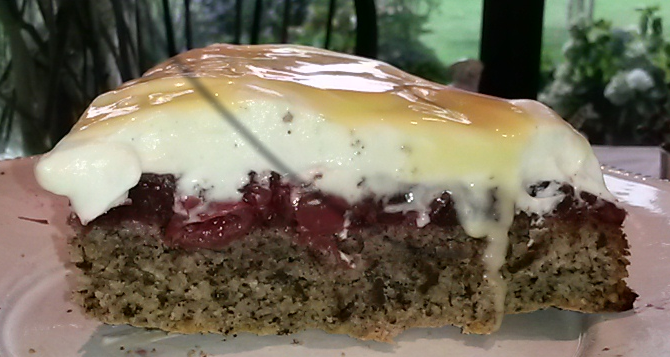
\includegraphics[scale=0.4]{pic}
\end{document}